\subsection{A limited test of a smooth-image trusted region}
\label{sec:smooth-trusted-region}
The preceding low-ink images are visibly atypical.  We therefore tested a separate, simple image restriction based on anisotropic total variation,
\[
 \operatorname{TV}(p)=\sum_{(i,j)\in\mathcal E}|p_i-p_j|,
 \qquad p\in[0,1]^{784},
\]
where $\mathcal E$ consists of horizontal and vertical nearest-neighbor edges.  The 10,000 official MNIST test images have median TV $102.55$, 99th percentile $143.74$, and maximum $180.41$.  These image statistics do not themselves establish that an input is natural.

For the fitted depth-16 full-MNIST model \texttt{105}, we minimized TV subject to zero first preactivations, a black two-pixel border, and mean ink at most $1/5$.  The resulting rounded eight-bit image remains a verified counterexample at $c=.001$, but its TV is $284.93$, above every test image.  This search therefore does \emph{not} refute a trusted region with TV at most $150$.

We can rigorously exclude this particular mechanism from that region.  An exact rational dual certificate gives
\[
 \operatorname{TV}(p)\ge284.87765209159
\]
for every image satisfying the stated border and ink constraints and exactly zero first preactivations.  More generally, the same certificate implies that an image in the border/ink region with TV at most $150$ has
\[
 \max_i |a_{1,i}|\ge0.1175517.
\]
These claims exclude zero and uniformly near-zero first states; they do not bound the later Jacobians or prove stability on the region.

A separately declared check gives the same qualitative conclusion for the fitted depth-$32$ model \texttt{301}.  Its exact rational dual certificate proves TV at least $287.04761391129$ for a zero first state under the same border and ink constraints.  TV at most $150$ instead forces maximum absolute first preactivation at least $.26750111067$.  None of the $4{,}097$ prescribed nearest and stochastic pixel-grid roundings of the numerical minimizer entered the region.  These are additional exclusions of this particular construction, not a uniform output-stability certificate or evidence that every fragile input has high TV.

For completeness, the certificate does not assume that the numerical linear-program solver is correct.  In normalized coordinates $x=2p-1$, introduce $t_e\in[0,2]$ with $\pm(x_i-x_j)\le t_e$, so TV is one half of the linear objective $\sum_e t_e$.  Write the resulting problem as minimizing $c^Ty$ with equality constraints $Ay=b$, inequalities $By\le d$, and coordinate box $l\le y\le u$.  For arbitrary exact dyadic multipliers $\lambda$ and $\mu\le0$, put $q=c-A^T\lambda-B^T\mu$.  Then
\[
 c^Ty\ge \lambda^Tb+\mu^Td+
       \sum_j\min\{q_jl_j,q_ju_j\}.
\]
We evaluate this expression using integer-rational arithmetic against the actual stored first-layer weights.  It remains valid even when the proposed dual multipliers are inaccurate.  If the equality constraint is violated by a first-preactivation vector $a_1$, the right side decreases by at most $\|\lambda\|_1\|a_1\|_\infty$; dividing by two gives the stated near-zero exclusion.  The exact coefficients and bound are saved for replay.

A complementary, separately declared stress test interpolated 256 deterministic opposite-parity pairs of correctly classified held-out MNIST images, using endpoints with TV at most $140$, ink at most $.195$, and black two-pixel borders.  We bisected toward output $0$ and $3/8$, rounded to eight-bit pixels, and retained all 512 rounded candidates satisfying TV at most $150$, ink at most $.2$, and the same border condition.  We attacked the 32 candidates with largest clean internal-noise gain for each target.  All 64 selected inputs pass the numerical finite-radius sufficient tests at $c=.001$ and $.003$, for both scores.  These are float64 evaluations of rigorous real inequalities, not interval proofs.  The corresponding attacks found no violations; that observation is not used as a substitute for the sufficient tests.

At $c=.01$, all 64 selected inputs have numerical primary-score violations.  Independently verified examples have TV $88.93$ and $100.13$, and mean ink $.118$ and $.158$.  To test disturbances confined to valid activation states, we set one offending noise coordinate to zero in each selected witness and reverified the resulting trajectories: all hidden states remain in $[-1,1]$, while the primary score changes by more than $.1474$ and the optional margin-band score changes by more than $.1384$, respectively.  The exact pixel sums verify the region constraints.  Figure~\ref{fig:tv-boundary-counterexample} shows one such interpolation.  Therefore a TV/ink restriction excludes the zero-state counterexample mechanism and improves this stress test at the smaller radii, but does not ensure the larger-radius condition.  No conclusion of uniform stability on the trusted region follows from these finite samples.

\begin{figure}[t]
\centering
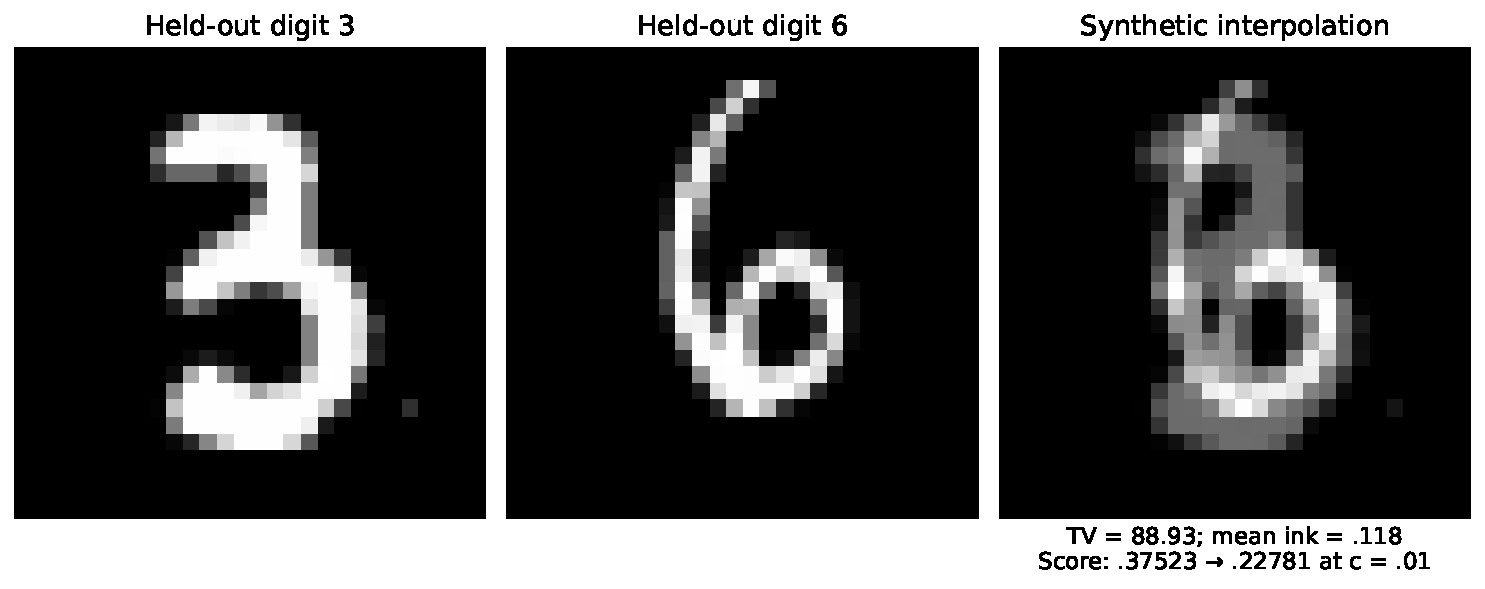
\includegraphics[width=.95\linewidth]{certificates/tv-boundary-counterexample.pdf}
\caption{An interpolation of opposite-parity held-out images, rounded to the eight-bit grid.  The interpolated image is synthetic and is not assigned a parity label.  At $c=.01$, a verified internal disturbance changes its clipped score by more than $.1474$, while every hidden state stays in $[-1,1]$.  Its TV and mean ink are within the stated smooth-image region.  This is a larger-radius example; the selected interpolation set passes numerical sufficient tests at $c=.001$ and $.003$.}
\label{fig:tv-boundary-counterexample}
\end{figure}
